\documentclass[a4paper,11pt]{article}

\usepackage{amsmath}
\usepackage{amssymb}
\usepackage{amsthm}
\usepackage{graphicx}
\usepackage{caption}
\usepackage{subcaption}

\newtheorem{thm}{Theorem}
\newtheorem{lem}{Lemma}

\newcommand{\beq}{\begin{equation}}
\newcommand{\eeq}{\end{equation}}

\newcommand{\ba}{\begin{array}}
\newcommand{\ea}{\end{array}}

\newcommand{\bea}{\begin{eqnarray}}
\newcommand{\eea}{\end{eqnarray}}

\newcommand{\bc}{\begin{center}}
\newcommand{\ec}{\end{center}}

\newcommand{\ds}{\displaystyle}

\newcommand{\bt}{\begin{tabular}}
\newcommand{\et}{\end{tabular}}

\newcommand{\bi}{\begin{itemize}}
\newcommand{\ei}{\end{itemize}}

\newcommand{\bd}{\begin{description}}
\newcommand{\ed}{\end{description}}

\newcommand{\bp}{\begin{pmatrix}}
\newcommand{\ep}{\end{pmatrix}}

\newcommand{\p}{\partial}
\newcommand{\sech}{\mbox{sech}}

\newcommand{\cf}{{\it cf.}~}

\newcommand{\ltwo}{L_{2}(\mathbb{R}^{2})}
\newcommand{\smooth}{C^{\infty}_{0}(\mathbb{R}^{2})}

\newcommand{\br}{{\bf r}}
\newcommand{\bk}{{\bf k}}
\newcommand{\bv}{{\bf v}}

\setlength{\textheight}{212mm}
\setlength{\textwidth}{165mm}
\topmargin -6mm
\oddsidemargin -6mm


\newcommand{\gnorm}[1]{\left|\left| #1\right|\right|}
\newcommand{\ipro}[2]{\left<#1,#2 \right>}
\title{Overshoot in Point-Vortex Approximations of Elliptical Vortex Patches}
\author{Chris Curtis, SDSU}
\date{}
\begin{document}
\maketitle
\section*{Model Setup}
In an inviscid, incompressible fluid, we can represent the fluid velocity ${\bf u}(x,z,t)$ generated by a vortex patch characterized by vorticity profile $\omega({\bf x},t)$ over the compact domain $\Omega(t)$ via the integral equation
\[
{\bf u}({\bf x},t) = \int_{\Omega(t)} {\bf K}({\bf x}-\tilde{{\bf x}})\omega(\tilde{{\bf x}},t)d\tilde{x}d\tilde{z},
\]
where $\omega$ is the vorticity, and ${\bf K}$ is the standard Biot-Savart law kernel; see \cite{saffman} for more details.  An attractive means for discretizing this equation as summarized in \cite{cottet} is to approximate the vorticity $\omega$ by a collection of $N$ point-vortices at positions ${\bf x}_{l}(t)$ via the expansion
\begin{equation}
\omega(\tilde{{\bf x}},t) = \sum_{j=1}^{N} \frac{\Gamma_{j}}{\delta^{2}}\chi\left(\frac{\tilde{{\bf x}}-{\bf x}_{l}(t)}{\delta}\right)
\label{discvort} 
\end{equation}
where $\chi$ is some appropriately chosen mollifier, see \cite{beale}, and $\Gamma_{j}$ is the circulation associated with the point vortex at ${\bf x}_{l}(t)$.  Thus, we can reduce the problem of tracking the evolution of the vortex patch to describing the motion of the point vortices via the system of ODE's
\[
\frac{d{\bf x}_{j}}{dt}  =  \sum_{l\neq j}^{N} \Gamma_{l} {\bf K}_{\delta}\left({\bf x}_{j}-{\bf x}_{l}\right) , ~ {\bf K}_{\delta}({\bf x}) = \frac{1}{\delta^{2}}\int_{\mathbb{R}^{2}}{\bf K}({\bf x} - \tilde{\bf x})\chi \left(\frac{\tilde{{\bf x}}}{\delta} \right) d \tilde{{\bf x}}.
\]

\section*{Numerical Experiments}
We now turn to the study of the Kirchoff elliptical vortices \cite{mitchell,crosby} and how their edge dynamics evolve in the above numerical scheme.  Above, a Kirchoff elliptical vortex is a vortex patch with constant vorticity $\omega$ and support within the elliptical disc
\[
\left(\frac{x}{a}\right)^{2} + \left(\frac{z-z_{c}}{b} \right)^{2} \leq 1.
\]
It is a now classical result, see \cite{mitchell} for details, that in the absence of outside influences, the patch simply rotates with $\dot{a}=\dot{b}=0$ and the angle describing the rotation being given in these coordinates by 
\[
\dot{\theta} = \frac{\omega ab}{(a+b)^{2}}.
\]
This is an idealized result however since if the ratio of major to minor axes is greater than three, the patch becomes unstable.  This instability manifests as the production of tendrils growing from the patch which, in a certain limit, provides an approximation to eventual vortex shedding.  The vorticity function is sampled over a uniform mesh of step size $dx = dz = 2.5 \times 10^{-3}$, and the initial circulations $\Gamma_{j}$ are found by solving the linear system in Equation \eqref{discvort}.  Note, this amounts to starting our simulation with $1596$ vortices within the patch.  We use a fourth order Runga-Kutta scheme with a time step of $dt = 10^{-1}$ and an integrating factor to address the dispersion introduced by the free-surface.  

We regrid the vortices to a uniform Eularian mesh every ten time steps to address the shear-induced distortion of the relative separation of the point-vortices.  To cope with the increasing number of vortices this introduces, we use a FMM to make the evaluation of the velocities induced by the vortices scale like $\mathcal{O}(N\log(N))$.  We note that in order to improve performance, we remove the mollification over the well-separated vortices in the FMM scheme, saving mollification only between nearest-neighbors in the FMM scheme.  The impact of this choice on the physics is negligible.  

To generate numerical simulations then, we model the vorticity as 
\[
\omega(x,z) = \omega_{0}\mbox{exp}\left(\log(\mbox{eps}) \left(\left(\frac{x}{a}\right)^{2} + \left(\frac{z-z_{c}}{b} \right)^{2}\right)^{n}\right)
\]
where $\mbox{eps}$ denotes machine precision, which is approximately $2\times 10^{-16}$ on 64-bit computers.  Note, this vorticity profile only has support on the original elliptical disc, has essentially constant vorticty $\omega_{0}$ throughout the elliptical disc, but smoothly vanishes at the boundary.  We can adjust the power $n$ so that as $n\rightarrow \infty$, we limit on to the discontinuous case, while for $n\rightarrow 0$, we generate a smooth patch with a relatively smeared boundary.  Thus, we can quantify the overshoot phenomena along the patch edge in terms of the regularity of the chosen patch.  

Choosing $a=2$, $b=1$, $\omega_{0}=1$, $z_{c}=.35$, and $n=18$, so that practically speaking we are in the discontinuous case, we get the following reconstruction of the vorticity after one iteration of our algorithm we generate the following solutions
\begin{figure}[!h]
\begin{tabular}{cc}
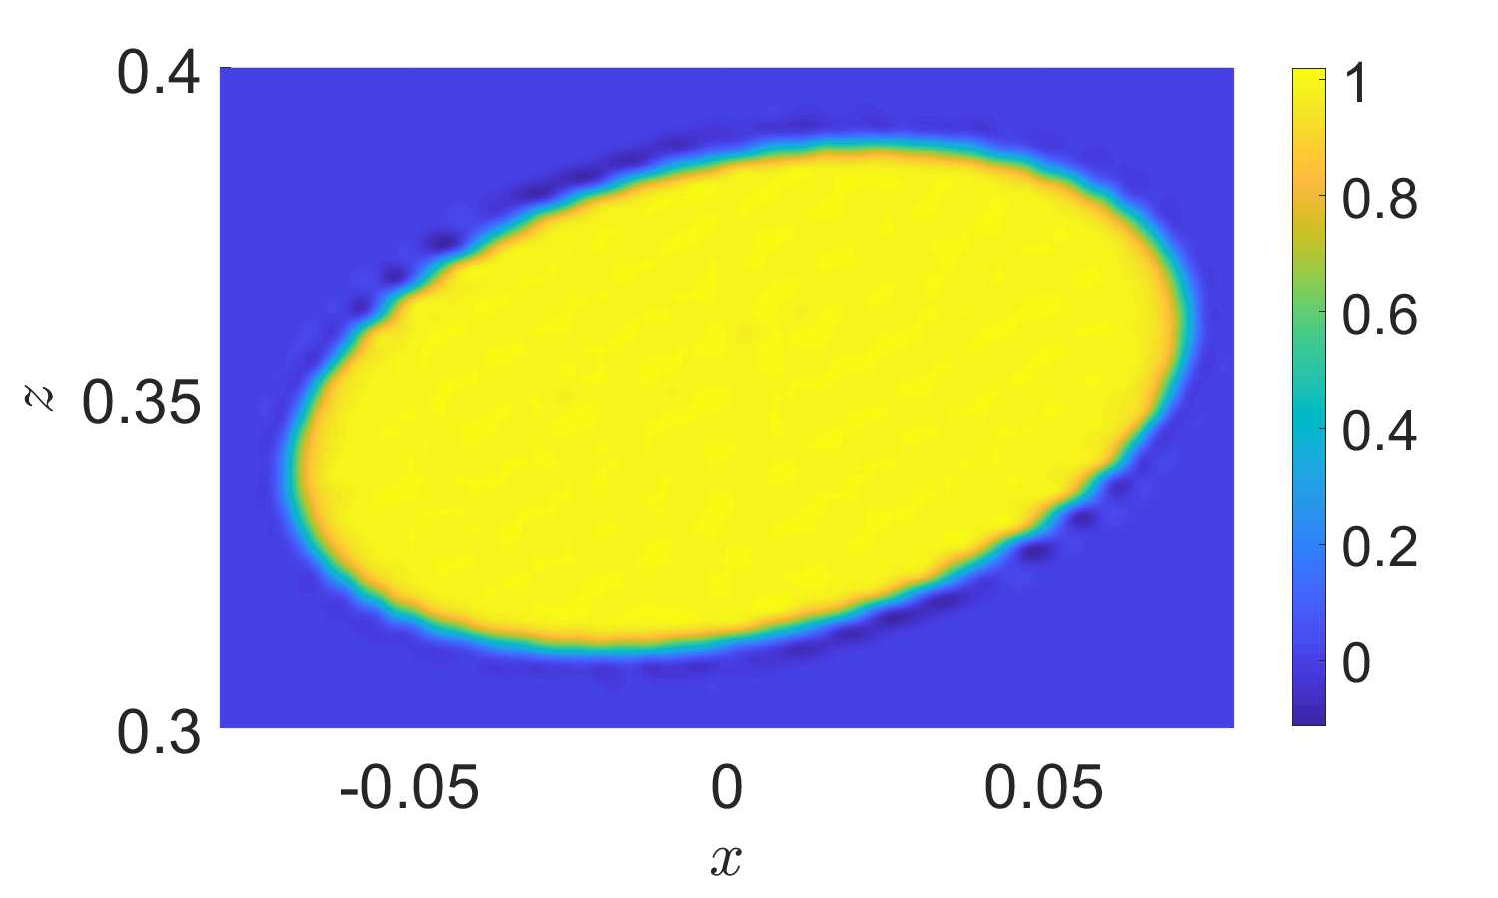
\includegraphics[width=.5\textwidth]{patch_reconstruction_n_18_w0_1} & 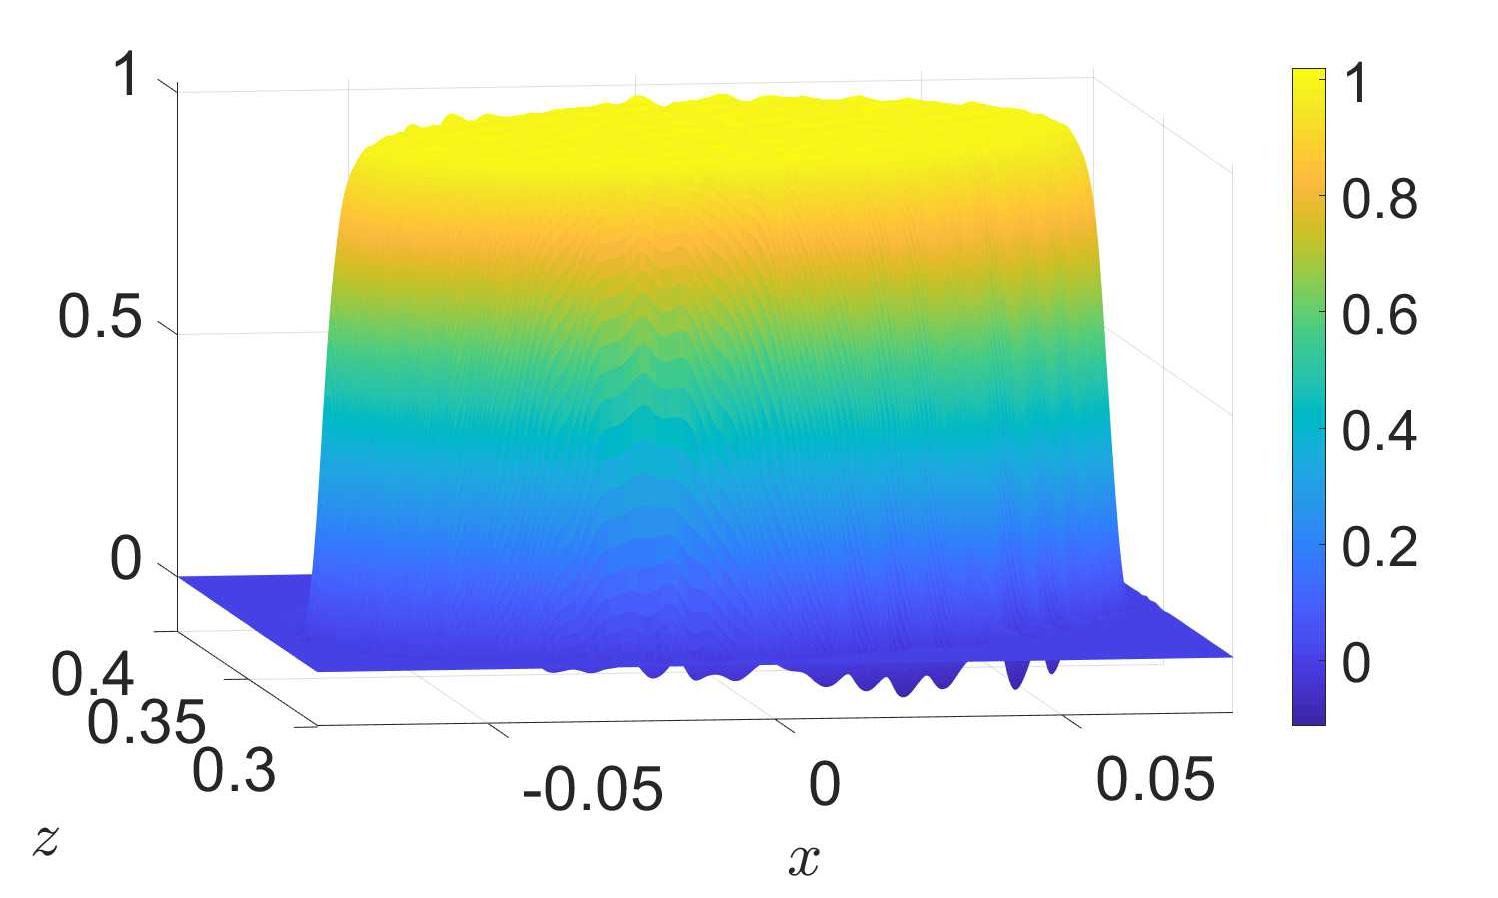
\includegraphics[width=.5\textwidth]{patch_reconstruction_n_18_w0_1_profile}\\
(a) & (b)
\end{tabular}
\caption{Reconstruction of an elliptical vortex patch with $a=2$, $b=1$, $\omega_{0}=1$, $z_{c}=.35$, and $n=18$, with a top-down view (a) and profile (b).  The numerical reconstruction is reasonably accurate within the interior of the patch, however oscillations at the egde are plainly visible representing significant interpolation error. }
\end{figure}
\bibliography{waves_over_vortices}
\bibliographystyle{unsrt}

\end{document}